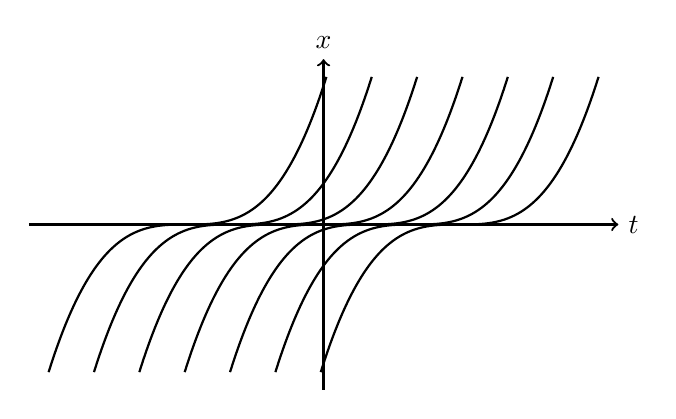
\begin{tikzpicture}[x=0.72cm,y=0.75cm,thick]
  \draw[->] (-5.2,0)--(5.2,0) node[right] {$t$};
  \draw[->] (0,-2.8)--(0,2.8) node[above] {$x$};
  \foreach \c in {-2.4,-1.6,-0.8,0,0.8,1.6,2.4} {
    \pgfmathsetmacro{\lo}{\c-2.45}
    \pgfmathsetmacro{\hi}{\c+2.45}
    \draw[domain=\lo:\hi,samples=90,smooth,variable=\t]
      plot (\t,{0.17*(\t-\c)^3});
  }
\end{tikzpicture}
